\documentclass[11pt]{article}
\usepackage{fullpage}
\usepackage{mathpazo}
\usepackage[noend]{algpseudocode}
\usepackage{amsmath}
\usepackage{latexsym}
\usepackage{graphicx}
\usepackage{wrapfig}
\usepackage{bibentry}
\usepackage{bm}
\usepackage{qtree}
\usepackage{array}
\usepackage{eurosym}
\usepackage{textcomp}
\usepackage{tocloft}
\usepackage{makeidx}
\usepackage{rotating}
\usepackage{multirow}
\usepackage{multicol}
\usepackage{microtype}
\usepackage[font=footnotesize,labelsep=quad,labelfont=it]{caption}
\newcommand\subcaptionsize\footnotesize  % make this the same as the font size in the caption package
\newcommand\ignore[1]{}

\renewcommand\textfraction{0.0}
\renewcommand\topfraction{1.0}
\renewcommand\bottomfraction{1.0}

\newcommand\tightbox[1]{{\setlength\fboxsep{0pt}\framebox{#1}}}

\sloppy
\raggedbottom

\begin{document}


\section*{Training Hierarchical Agent Behaviors for Games or Robotics\\{\large White Paper}}

\subsection*{Vittorio Ziparo and Sean Luke}

We are experimenting with an approach to training agents, and ultimately swarms of agents, for complex behaviors, using learnable hierarchies of finite-state automata.

This work involves various technologies and methods, some of which have been well studied in the past; but to the best of our knowledge our approach is novel and pretty ambitious in scope.  If successful (and that's a big if), we think it could have a significant impact.

\subsection*{Motivation}

We've both done a fair bit of work in robotics, agents, and multiagent systems.  Vittorio got his PhD in robotics with a particular emphasis on agent-based behaviors.  His PhD work involved the design of an agent planning framework based on Petri nets.  Sean has done a variety of multiagent and robotics work, with a strong emphasis on emergent behavior arising from simple agent behaviors, and also on the application of machine learning and evolutionary optimization to the development of such behaviors.

In robotics, it can be challenging to design sophisticated plans and to reason over them.   Furthermore, multiagent plans present additional difficulties due to possible macrophenomena emerging from the interactions of agents with even simple behaviors.  Much robotic behavior learning research has focused on optimization methods (such as evolutionary algorithms) or reinforcement learning.  Though some work exists in the use of supervised learning to assist in the development of agent behaviors, using supervised learning for entire agent plans is relatively rare.

The situation in games is surprisingly similar to that in robotics: and not surprisingly �the techniques and tools used in robotics transfer to game development handily.  

Our primary interest is in training agents to learn behaviors, then store those behaviors as functions which can be used in higher-level training.  We think this would be of interest to the robotics community; to the agent behavior community (for example, people developing agent behaviors for games or computer graphics purposes); and it might also make an interesting (if perhaps not fun!) game in and of itself: we envision a game called {\it Guru} or {\it Horde} in which the player's job is to train his minions in simple, then advanced, tasks until they can wage war against other minion armies (from other players).
 
\subsection*{Prior Work}

Unlike much of the literature, we are doing supervised learning.  The most famous example, to our knowledge, of supervised learning used for agent behaviors is Peter Stone's dissertation \cite{stone}, in which he used various machine learning methods (notably backpropagation and decision trees) to learn explicit layers of certain soccer behaviors.

Much remaining work is either reinforcement learning or evolutionary computation rather than a supervised method.  Among the most similar approaches to ours is Yasutake Takahashi and Minoru Asada's work on using reinforcement learning to discover modules which can then be used as events for higher-level learned modules \cite{yasutake1}.  The two have also recently extended this to using these modules to decompose (in a top-down fashion) a behavior acquired by watching a ``coach'' perform the action \cite{yasutake2}.  Curiously these methods use reinforcement learning even though coach information etc. is essentially supervised: the methods are throwing away information.

At this stage the work we're doing is exploratory and experimental: and we harbor no doubt that the literature on this topic is deep and what we're doing so far has been done before many times.

\subsection*{Agent Behavior Model}

Our agent model is based on a simple collection of Mealy-machine style finite state automata.  Each automaton in the collection contains a collection of {\it states} \(S\) connected by some number of {\it transition edges} \(E\).  One state is designated the {\it start state}.  Each state denotes a behavior: while the agent is in state \(s\in S\), it is doing the behavior associated with \(s\).  The automaton may also have some number of special states called {\it ``done'' states}, indicating that the action is completed.  ``Done'' states do not have an associated behavior per se.

When in a given state \(s\), the agent may follow along a transition edge \(e\) connecting \(s\) to some other state \(s'\). This edge is labeled with a {\it condition} indicating what must be true about the world in order to transition along that edge.  For example, an agent may be in the state ``CleanUpRoom'' until the condition ``UserEnteredRoom'' becomes true, at which time the agent transitions along that edge to the new state ``HideUnderBed''.  These conditions don't have to be boolean symbols necessarily: they could be things like ``Room is 70\% Cleaned Up'' or ``Bed is less than 20 feet away and light is not turned on''.  If no outgoing edge from \(s\) exists whose condition is presently true, we stay in \(s\) and continue to do its behavior.

Straightforward so far!  We augment this model with two additional gizmos:

\begin{itemize}
\item A hierarchy among state machines.
\item A transition model.
\end{itemize}

\paragraph{Hierarchy}  The states \(S\) in a state machine are actually of one of two possible kinds: {\it atomic states} and {\it macro states}.  Atomic states denote hard-coded basic agent behaviors.  Macro states denote behaviors which are actually {\it other FSAs}.  When we transition to a macro state \(m\), we push the present FSA on a stack and start executing the {\it macro FSA} associated with \(m\).  We begin in the ``start'' state of this macro FSA.  This action is recursive: if in this macro FSA we encounter a macro state, we push it on the stack and start executing that other macro FSA, and so on.

When the macro FSA reaches a ``done'' state, the FSA is popped off the stack and we return to the parent FSA, and signal the transition condition ``Done''.  If there is an outgoing edge from \(m\) for this condition, we transition from \(m\) to a new state along this edge.  If not, we once again execute \(m\): pushing the FSA on the stack, and once again executing \(m\)'s macro FSA starting at the ``start'' state.

While executing \(m\)'s macro FSA, the parent FSA isn't frozen {\it per se}: if a condition arises for which there is an edge out of \(m\), we immediately exit the macro FSA and return to \(m\) and transition from there.  This is the case for all parents: we wander up the stack to the highest-level parent for which this is the case.  The only exception is the ``done'' condition, which is only visible to the immediate parent.

The point of a macro hierarchy among FSA is to enable the construction of behavior libraries.  For example, we might build a simple FSA called {\it Wall-Follow}, and another FSA called {\it Go-To-Target}.  We can then use these FSAs as macros in a higher-level FSA which implements an (incorrect) version of  the so-called robotics {\it Bug-Algorithm}: go to the target until you hit an obstacle.  Then wall-follow around that obstacle until you are in line with the target again, at which time go after the target again.  

Hierarchical FSAs are not new: for example, their use in robotics includes work by Monica Nicolescu and Maja Matari{\'c} \cite{mataric}.  Sean Luke and his student Randy Steck also developed a Java-based robot framework for robotics.  Furthermore, Vittorio Zipparo developed a hierarchical petri net framework for defining parallel robot plans \cite{ziparo}.

\paragraph{Transition Model}  Our primary interest is in training FSAs rather than explicitly coding them.  To this end we have a different model for the edges leaving \(s\).  Let the full set of outgoing edges from \(s\) collectively be called \(E_s\).  Rather than have individual edges, we could instead replace them with a {\it classification model} such as a decision tree or support vector machine.  The attributes of the model are various conditions and the classes of the model are other states led to by edges in \(E_s\), plus \(s\) itself.  We feed into the model the current world condition, and it tells us what new state \(s'\) to transition to.  In many situations, \(s'\) may be \(s\) itself, indicating that we shouldn't do a transition for now.  This model might be deterministic or probabilistic.  Viewing the edges as a model like this allows us to then {\it learn} a transition model for \(s\) during the training step discussed later.

\subsection*{Implementation}

\begin{wrapfigure}{r}[0in]{2.5in}
\vspace{-1em}
\tightbox{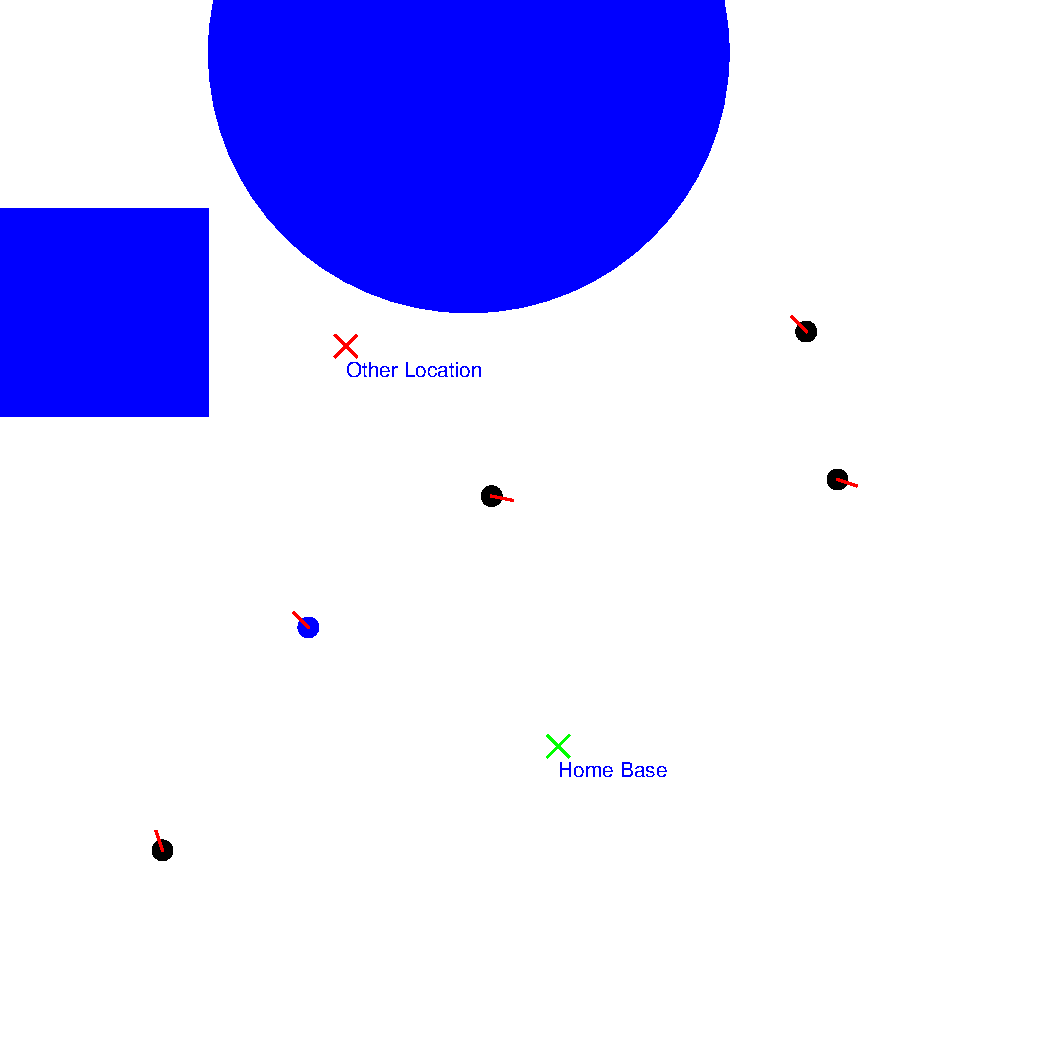
\includegraphics[width=2.5in]{Horde.pdf}}
\vspace{-1em}
\caption{A scenario in Horde.}
\label{horde}
\end{wrapfigure}

We have implemented a testbed for research of this kind, with a new application called {\it Horde}, written using the MASON multiagent simulation toolkit \cite{luke:simulation:2005} (see http://cs.gmu.edu/\(\sim\)eclab/projects/mason/).  MASON was written by Sean Luke and so it's convenient to us!  It also has the benefit of being specially designed for tasks of this nature.  MASON supports 3D graphics and models as well, but to keep things simple we're sticking with trivial 2D worlds right now, and with a point object representing our agent, various obstacles and other agents, and various waypoints.  In the environment, our agent can sense various things: the relative locations of obstacles, other agents of different classes (perhaps members of his immediate team, or opponents, or random agents), certain predefined waypoints, etc.  The agent can also sense situations which may have changed in the world.  We're flexible for now.

\subsection*{Training Agents}

\begin{wrapfigure}{r}[0in]{2.5in}
\vspace{-3em}
\hspace{-0.7em}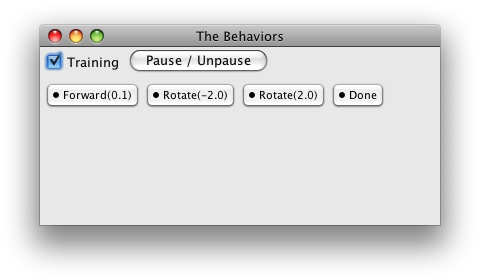
\includegraphics[width=2.8in]{Behaviors.png}
\vspace{-3em}
\caption{A simple behavior control window.}
\vspace{-4em}
\label{behavior}
\end{wrapfigure}

Our approach to training agents is to start with a set of possible behavior states, including a start state and a single ``done'' state.  Each behavior state has a transition model, initially empty, meaning that initially when in a given behavior the agent never transitions to any other.  Our current transition models are decision trees.

Figure \ref{behavior} shows a simple behavior panel with four behaviors (Forward, Rotate left, Rotate right, and Done).  As the simulation progresses the user may press on certain buttons to direct the agent to take different behaviors in an attempt to show the agent the user's desired course of action.  For example, to circle around the ``Home Base'' target, the user may press the Forward and Rotate Left buttons as necessary.  Each button represents a behavior state in the system.  When the user presses a button, the FSA transitions to that state.  At this time, and possible at certain other times, the system samples the world situation and stores an examplar \(\langle s, w, s' \rangle\), indicating that when in state \(s\), and when the world looked like \(w\) to the agent, the user asked transition to new state \(s'\).  From these examplars we can then build up a decision tree for each state \(s\).  Specifically, for each state \(s_i\), we transform all examplars of the form \(\langle s_i, w, s' \rangle\) into simple input-output data pairs \(\langle w, s'\rangle\) for a decision tree, where \(w\) is the input (the attribute vector) and \(s'\) is the output (the decision tree class).  We also include collect world samples of the form  \(\langle s_i, w, s_i\rangle\), that is, situations where no transition occurred, and include those as well: \(\langle w, s\).  From this we can build a model which learns, for any given state and world situation, what to do next.  When the user unchecks the ``training'' checkbox, ideally the agent should perform the behavior in a general fashion.

One interesting item we've been experimenting with: probabilistic class results from the decision tree.  Usually decision trees have deterministic classes as their leaf nodes (``definitely transition to {\it turn-right}''), because in most machine learning situations the output is a single desired class.  But in our scenarios it's often desirable to have probabilistic outputs ({\it ``turn-right'' 90\% of the time, ``go-forward'' 10\% of the time}) based on the samples gathered.

\subsection*{Problems to Tackle Still}

Our initial scenario appears to work: we can train agents to perform simple tasks such as wall-following, acquiring a target, circling a target, etc.  But we have a number of things to tackle yet:

\paragraph{Aliased Behavior States}

Note that our present design assumes that there is a {\it single state} for each behavior.  To be maximally general, an FSA should allow any number of states for a given behavior.  Wall-following is an example: there are two situations where one needs to move {\it forward} (initial movement; and when going down a wall).  At present we only allow a single {\it forward} state, though in these situations it's possible to require different outgoing transitions for these two situations.  One easy way to fix this is to ``train'' a behavior consisting solely of moving {\it forward}.  Call this new behavior {\it forward2}.  We can then include both {\it forward} and {\it forward2} as states in a higher environment. 

We also often have aliased situations.  For example, in the wall-following scenario the agent may find itself unable to see anything in front or to the side of it (assuming it only has front and side sensors).  This could happen initially when the agent is in an arbitrary location --- in which case the agent should move forward --- or it could happen when the agent has wandered off of a tight outer turn --- in which case the agent should turn right.  However our present FSA model, at least in limited cases, handles such aliased situations without much difficulty.  We think!

\paragraph{Continuous Attributes}

Our initial tests have assumed categorical attributes (that is, using IB3 as the decision tree), but any serious use will require continuous attributes (something like C4.5) and pruning.  We're building that in as we speak.

\paragraph{Parameterized FSAs and the Sensing Problem}

If you have a macro behavior like ``attack the bad guy'', and wish to use it in a higher-level FSA, you will need to be able to specify {\it which} bad guy to attack.  This isn't something built into normal FSAs.  We're experimenting with a design where you can specify up to some \(M\) {\it generic targets} (in Figure \ref{horde} the targets are denominated with X's).  The behavior can then be done with respect to those targets, or with respect to certain other {\it relative targets} (``the closest neighbor to me'', for example).  In the higher-level FSA, when you transition to the state \(m\) which expands to this macro FSA, you'll need to specify what those generic targets are, in the context of the higher-level FSA.

This essentially allows parameters of a sort.  Allowing parameters moves us away from training and towards direct programming; which may be a necessary evil but, for purposes of this research, is probably an evil nonetheless.  Another factor which moves us towards direct programming: the sensing problem.  Having a great many behaviors available isn't a problem.  But having a great many sensors, and resulting world attributes and situations, {\it is} a problem.  With too many sensor values, training the system to ignore the ones that shouldn't matter takes a lot more training cycles.  We could trim it to just a few sensor values, but run the risk of not having enough sensors to learn the problem.   Ultimately, specifying which sensors should be used for a given behavior (which would solve the problem) moves us directly towards programming the behaviors.  We have ideas regarding learning which sensors matter and which do not, but they're nontrivial and may be discarded.

\paragraph{Multiagent Training and Stochastic Optimization}

Ultimately our goal is to train emergent multiagent behaviors.  We have given very little thought about how to go about doing this in a supervised fashion.  Ultimately we may need to resort to stochastic optimization techniques such as evolutionary computation (possibly using ECJ (http://cs.gmu.edu/\(\sim\)eclab/projects/ecj), which dovetails with MASON). 

We are interested in constructing hierarchies among the agents.  This is not to be confused with behavior hierarchies as discussed so far.  Rather, agents would be grouped into teams, each with an agent leader, and the leaders would be grouped into teams, and so on up to a top-level directed by the user.  Agents in a team can raise conditions which are sensed by their leader (we'd train this), and the leader can also raise conditions which cause state transitions among his subordinates.

\paragraph{More Compelling Test Scenarios}

Though elements of this work have been done before in other guises, we are not aware of any work which has attempted to put this together on a scale of this magnitude.  In order to drive efforts in these areas, and work out kinks we'd not considered, we need test scenarios to challenge us.  This is harder than it sounds!

% declare bibliographic entries which can get stuck in footnotes etc.
\bibliographystyle{notes}
\bibliography{whitepaper}

\end{document}